\documentclass[varwidth=\maxdimen]{standalone}
\usepackage{diagbox}
\usepackage{rotating}
\usepackage{tikz}
\usetikzlibrary{calc}
\begin{document}

    \begin{table}[h!]
        \begin{center}
            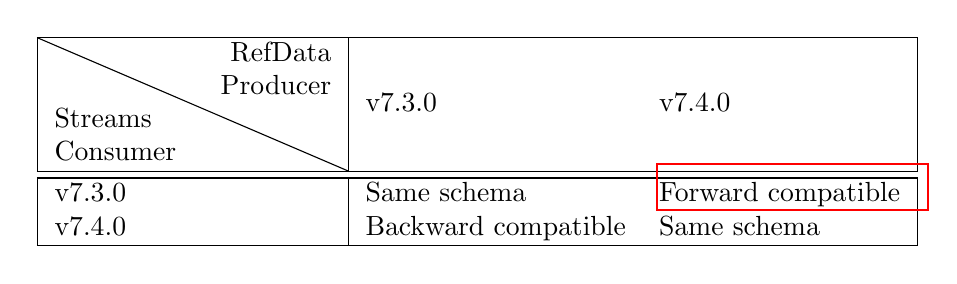
\begin{tikzpicture}\node (table) {
                \begin{tabular}{|l|ll|}
                    \hline
                    \diagbox{Streams\\Consumer}{RefData\\Producer} & v7.3.0 & v7.4.0 \\
                    \hline
                    \hline
                    v7.3.0 & Same schema & Forward compatible \\
                    v7.4.0 & Backward compatible & Same schema \\
                    \hline
                \end{tabular}};
            \draw [red,thick]
            ($(table.south west) !.2! (table.north west) + (8,0)$)
            rectangle
            ($(table.south east) !.4! (table.north east)$);
            \end{tikzpicture}
        \end{center}\label{tab:table}
    \end{table}


\end{document}